\documentclass[11pt]{article}
\usepackage[margin=1in]{geometry}
\usepackage[utf8]{inputenc}
\usepackage[T1]{fontenc}
\usepackage{amsmath,amssymb}
\usepackage{booktabs}
\usepackage{graphicx}
\usepackage{microtype}
\usepackage[round]{natbib}
\usepackage[hidelinks]{hyperref}
\usepackage{caption}
\captionsetup{font=small,labelfont=bf}
\graphicspath{{../results/}{figures/}{./}}

\newcommand{\E}{\mathbb{E}}

\title{\bfseries De-censoring Has a Ceiling, and It Is Low:\\
an Information Bound for Censored Retail Demand}
% Draft v4 --- submission candidate, content freeze 2026-11-20.
% TODO before submission: author block, affiliation, corresponding author.
\author{[First Author]\\[2pt] [Affiliation]\\[2pt] \texttt{[email]}}
\date{}

\begin{document}
\maketitle

\begin{abstract}
\noindent
Retail demand is censored by inventory, and a 2025--2026 literature on the
FreshRetailNet-50K benchmark competes on forecast accuracy. We ask how much
accuracy is available. A censored day does not carry a clean day's information,
and we compute the shortfall exactly: at the benchmark's mean severity of 0.32,
a censored day retains 22--58\% of a clean day's Fisher information, 90 days of
data are worth about 68 (25\% destroyed), and the Cram\'er--Rao floor on the
standard error of any unbiased per-SKU level estimate is a median 7.0\%. Against
a daily coefficient of variation of about 25\%, a 7\% level uncertainty is a
minor term---which explains a pattern the field reports without explaining:
eleven methods, spanning linear interpolation to ImputeFormer, differ by 35
percentage points in bias and, with the bias removed, by only 1.1 in WAPE;
$|\text{bias}|$ alone correlates with 89\% of the between-method WAPE
variance---a correlation that, on inspection, is not causal. Once the bias is
corrected the error sits at a floor near 20 WAPE, and no method has gone below
it. The decision layer is not bounded in the same way: ordering at the newsvendor
quantile rather than the mean moves lost units by $16.8\times$ on its own
($18.7\times$ once the history is de-censored), an order of magnitude more than
the entire reconstruction question. De-censoring is worth doing to remove bias;
it is not worth funding to chase accuracy.
\end{abstract}

\section{The claim}

Two literatures describe the same defect. Operations research calls it
\emph{unconstraining} and estimates a demand distribution from censored sales
\citep{nahmias1994,talluri2004,vulcano2012,tobin1958,kaplan1958}. Machine
learning calls it \emph{latent demand recovery} and imputes the missing days
\citep{du2023,wu2023,nie2024}. Both are judged by forecast error. On
FreshRetailNet-50K \citep{wang2025} the recent reports are: bias moving from
$-8.23\%$ to $-2.62\%$ with inverse-Mills-ratio recovery \citep{azar2026};
$-8.1\%$ to $-1.3\%$ with an hourly censoring-aware model \citep{cadre2026}; and
a relational model finding that recovery alone does not improve WAPE
\citep{chen2025}.

Bias moves a lot; accuracy moves a little. That pattern is not a property of the
methods. It is a property of the information the censoring left, and this paper
measures it.

\paragraph{Claim.} The accuracy gains available from de-censoring are bounded by
how much information the censoring left, and that bound is low. The bias is the
part that is both large and removable; the residual error is neither.

\paragraph{What this paper is, and is not.} It is not a new reconstruction
method, and it does not claim to beat any of the eleven it compares---on this
protocol it wins by $0.2$ points, and says so. It is an accounting paper: it
computes what the censoring destroyed, prices the residue in the metric the field
optimises, and shows that the differences the field reports are the part the
bound leaves free. The method slot on this benchmark is already occupied three
times over, which is why a fourth estimator is the wrong contribution here
(Table~\ref{tab:prior}).

\begin{table}[t]
\centering\small
\caption{What occupies the method slot on FreshRetailNet-50K, and what each
leaves open.}
\label{tab:prior}
\begin{tabular}{@{}p{2.6cm}p{4.3cm}p{4.1cm}p{4.1cm}@{}}
\toprule
work & what it reports & what it occupies & what it leaves \\
\midrule
Azar 2026 \citep{azar2026} & inverse-Mills ratio; bias $-8.23\%\to-2.62\%$; a
leakage-free pipeline & a working method, an evaluation protocol & no bound on
what remains \\
Yin et al.\ 2026 \citep{cadre2026} & stock-out flags as lower bounds; hourly
separation of censoring & censoring-aware feature engineering & no accuracy
ceiling \\
Chen \& Jin 2025 \citep{chen2025} & relational model; recovery alone does not
improve WAPE & the observation this paper formalises & no quantification of
why \\
\bottomrule
\end{tabular}
\end{table}

The last row is the one to keep in view: the field has already noticed that
recovery does not buy accuracy. What it has not done is compute how much accuracy
was ever there to buy. That is the whole claim, and \S4 states the two ways it
can be falsified.

\section{How much information a censored day carries}

For a day observed with stock level $c$, the observation is a mixture: values
below $c$ are seen exactly, values at or above $c$ collapse into the event
$D \ge c$. Under a demand family $p(\cdot;\mu)$ the Fisher information about
$\mu$ is
\begin{equation}
I(c,\mu)=\sum_{y<c}p(y)\left(\frac{\partial\log p(y)}{\partial\mu}\right)^{2}
+ P(D\ge c)\left(\frac{\partial\log P(D\ge c)}{\partial\mu}\right)^{2},
\end{equation}
and the \emph{retention} $\rho=I(c,\mu)/I(\infty,\mu)$ is the fraction of a clean
day's information that survives. Under negative-binomial demand, $\rho$ depends
on the level $\mu$ and on the severity $s$ (the fraction of volume unreachable,
which fixes $c$ through $\E[\min(D,c)]=(1-s)\mu$).

\begin{figure}[t]
\centering
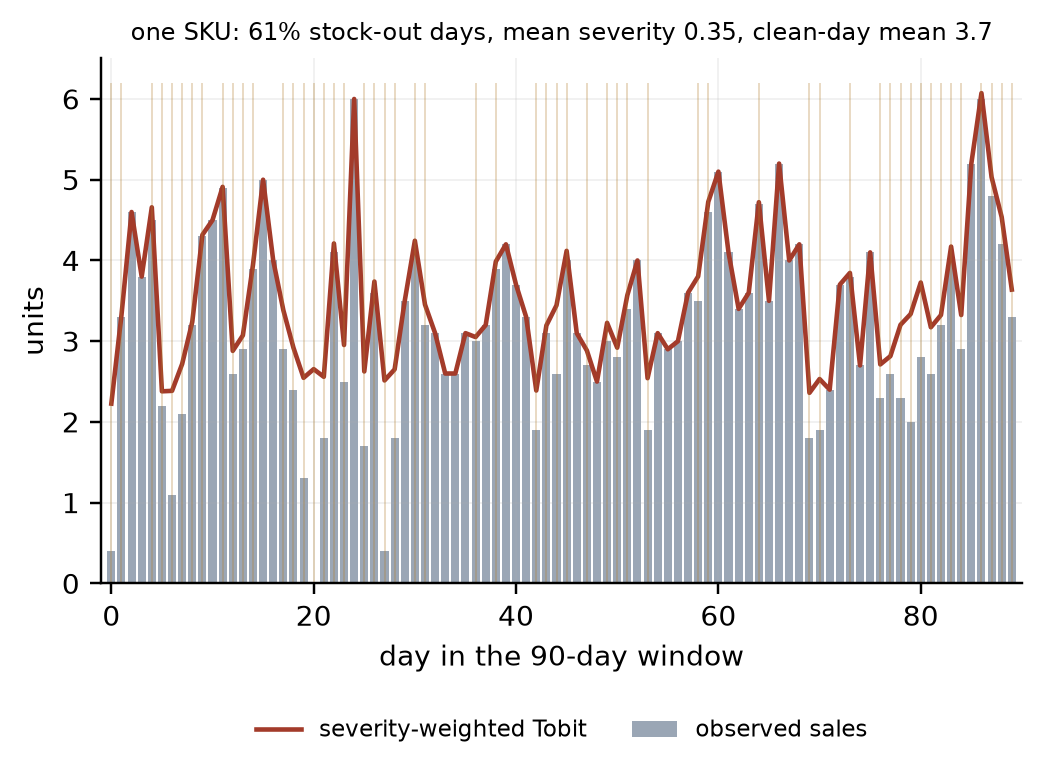
\includegraphics[width=.85\linewidth]{p5_example_series.png}
\caption{The problem in one picture: one SKU with 61\% stock-out days and a mean
severity of 0.35. Bars are recorded sales, the line is the severity-weighted
reconstruction, and the thin vertical lines mark stock-out days. The
reconstruction adds 9.0\% over the window, on exactly the days the bars are
short---and the demand it restores was never observed, which is why \S3 scores
only fully-stocked days.}
\label{fig:example}
\end{figure}

\begin{figure}[t]
\centering
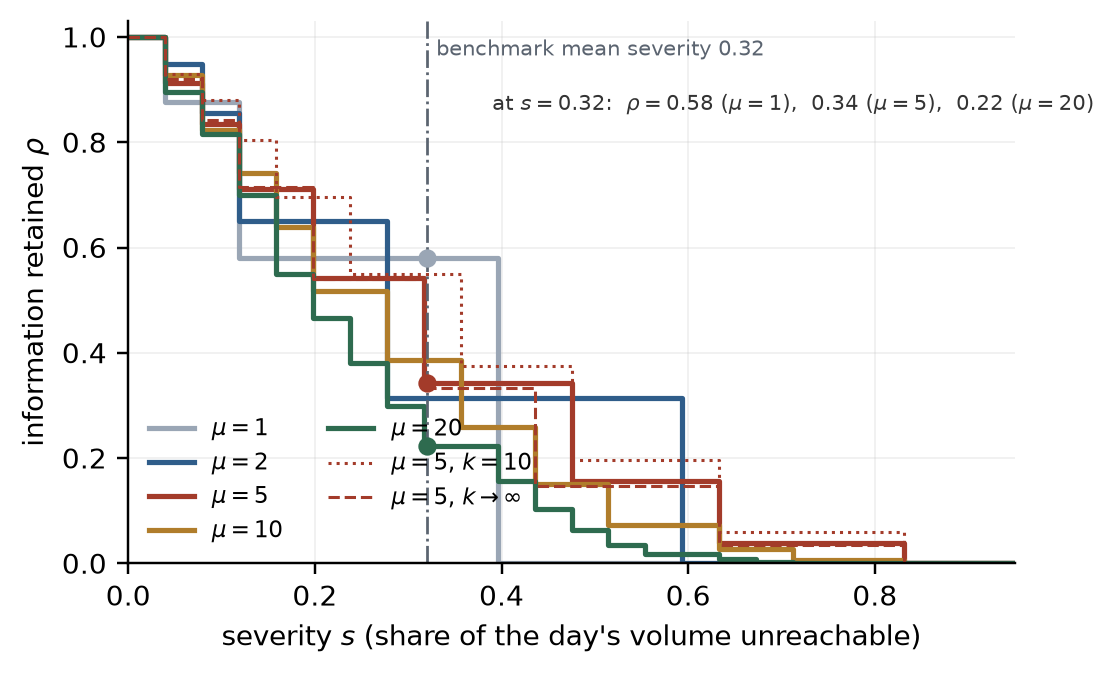
\includegraphics[width=.8\linewidth]{p1_information_curves.png}
\caption{Information retained by a censored day. Retention is a step function of
severity because demand is integer: whenever the implied stock level crosses an
integer, the censoring event changes and $\rho$ jumps. The markers are the values
quoted in the text, at the benchmark's mean severity.}
\label{fig:info}
\end{figure}

Retention is a \emph{step} function of severity, not a smooth one, because demand
is counted in whole units: every time the implied stock level crosses an integer
the censoring event changes and $\rho$ jumps (Fig.~\ref{fig:info}). At $s=0.32$,
the benchmark's mean severity, $\rho$ is 0.58 at $\mu=1$, 0.34 at $\mu=5$ and 0.22
at $\mu=20$ (marked). Dispersion matters much less than the level: at $\mu=5$ and
$s=0.32$, $\rho$ moves only from 0.374 ($k=10$) to 0.334 ($k\to\infty$), so the
bound is robust to a mis-specified tail. The computation is exact and we validate
it against Monte Carlo estimation of the score variance (agreement to $10^{-3}$ on
five settings).

\section{Accounting on the benchmark}

We sample 1{,}500 of the 50{,}000 series (52.7\% stock-out days) and compute per
series the effective sample size $n_{\text{eff}}=\sum_t \rho(s_t)$ and the
Cram\'er--Rao floor on the relative standard error of the level,
$1/\sqrt{n_{\text{eff}}I_1(\mu)}/\mu$.

\begin{table}[t]
\centering
\small
\caption{Information accounting per series (medians over 1{,}500 SKUs).}
\label{tab:acct}
\begin{tabular}{lr}
\toprule
quantity & median \\
\midrule
nominal days & 90 \\
clean days & 44 \\
\textbf{effective days} & \textbf{67.8} \\
information destroyed & 24.7\% \\
CR floor on level SE & 7.0\% \ (p90 8.3\%) \\
\bottomrule
\end{tabular}
\end{table}

Censoring destroys a quarter of the level's information. The floor on a
series-level estimate is 7\%.

\begin{figure}[t]
\centering
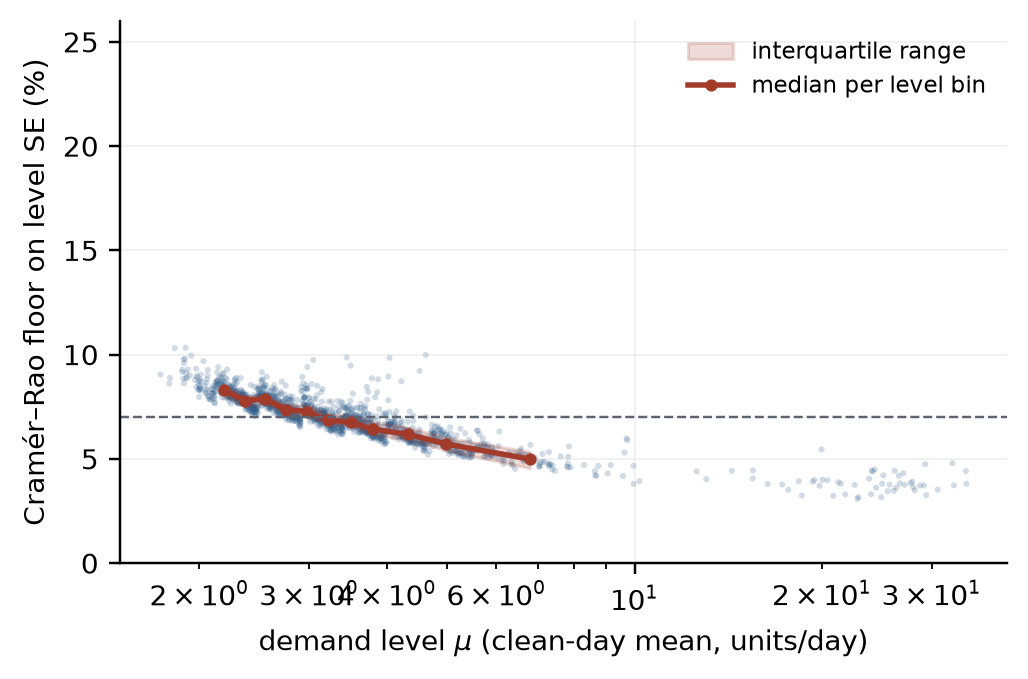
\includegraphics[width=.8\linewidth]{p2_bound_vs_level.png}
\caption{The floor is not one number across the panel: it falls from about 8.0\%
for the slowest quartile of series to 5.5\% for the fastest, because a
low-volume SKU carries less information per day to begin with. The panel is drawn
from the heavy end of the catalogue, so the 7\% median is a lower bound for a
real catalogue rather than a typical value.}
\label{fig:level}
\end{figure}

The floor is not one number across the panel (Fig.~\ref{fig:level}): it falls from
about 8.0\% for the slowest quartile of series to 5.5\% for the fastest, because a
low-volume SKU carries less information per day to begin with. Within this panel
only 0.2\% of series exceed a 10\% floor---a fact worth stating plainly, because
the panel is drawn from the heavy end of the catalogue (the 4{,}000 best-selling
series). The long tail, where a series sells a few units a week, is absent here
and would sit strictly above these curves; the 7\% floor is therefore a
\emph{lower} bound for a real catalogue. That is the conservative direction for a
ceiling claim, and the opposite direction for a practitioner carrying many slow
movers.

\section{The ceiling is visible in the numbers}

\begin{table}[t]
\centering\small
\caption{All eleven methods on the official holdout. \emph{fill} and \emph{lost}
are the inventory simulation of \S5 (50:1 cost ratio, 3-day lead time); the two
deep models are reported on accuracy only. A TimesNet baseline collapsed to 28.0
WAPE ($-13.6\%$ bias) after normalisation and is quoted in the text rather than
here. The full run takes 300\,s on a laptop CPU.}
\label{tab:methods}
\begin{tabular}{lrrrr}
\toprule
method & WAPE & bias & fill & lost \\
\midrule
sales as demand & 23.4 & $-7.1\%$ & 0.865 & 6154 \\
linear interpolation & 21.1 & $+1.3\%$ & 0.898 & 4643 \\
gradient-boosted imputation & 21.3 & $+1.6\%$ & 0.901 & 4496 \\
Kaplan--Meier (hard) & 28.8 & $+9.4\%$ & 0.899 & 4602 \\
Tobit (hard) & 23.3 & $+10.6\%$ & 0.934 & 3023 \\
negative binomial (hard) & 35.9 & $+28.0\%$ & 0.960 & 1815 \\
Kaplan--Meier (severity) & 22.1 & $+3.2\%$ & 0.899 & 4604 \\
Tobit (severity) & \textbf{20.5} & $\mathbf{-0.3\%}$ & 0.896 & 4723 \\
negative binomial (severity) & \textbf{20.3} & $+1.5\%$ & 0.906 & 4271 \\
SAITS (4 runs) & 21.4 & $+2.1\%$ & -- & -- \\
ImputeFormer & 20.4 & $+4.3\%$ & -- & -- \\
\bottomrule
\end{tabular}
\end{table}

Table~\ref{tab:methods} puts all eleven methods in one place, on the official
holdout. They span 20.3 to 35.9 WAPE and $-7.1\%$ to $+28.0\%$ bias, and the two
axes are not independent: across the eleven,
$\mathrm{corr}(|\text{bias}|,\text{WAPE})=0.94$ ($R^2=0.89$) with a fitted slope
of 0.56 WAPE per point of absolute bias (Fig.~\ref{fig:plane})---almost all of the
accuracy difference between methods \emph{is} their bias difference.

\begin{figure}[t]
\centering
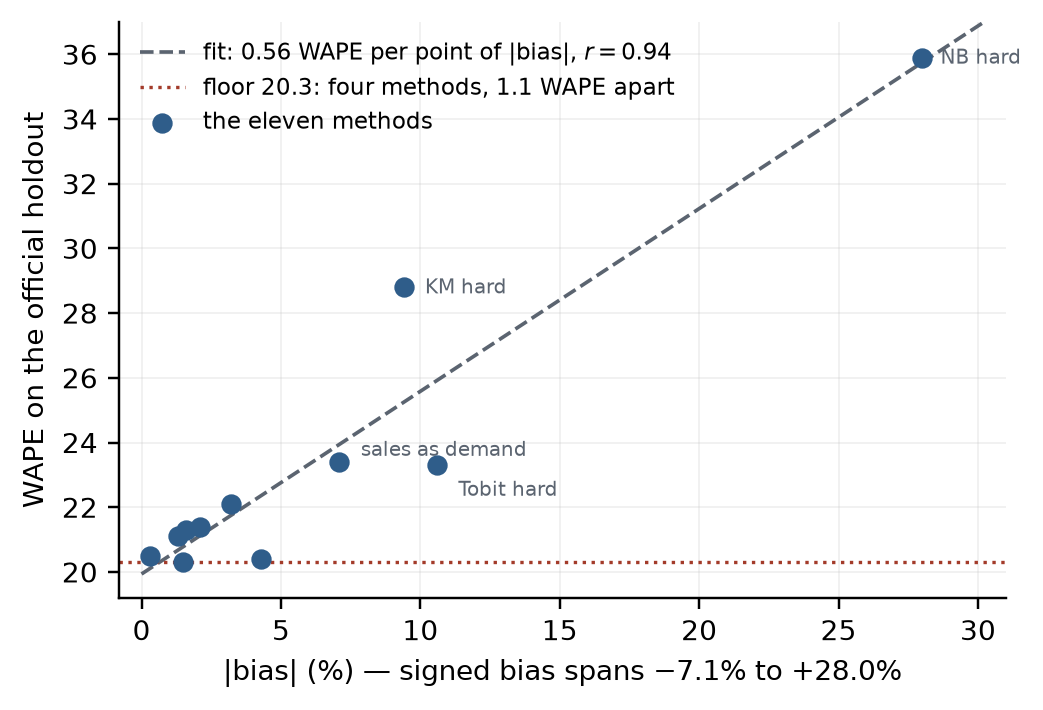
\includegraphics[width=.8\linewidth]{p4_bias_accuracy.png}
\caption{Bias against accuracy, all eleven methods. The four methods at the floor
span 1.1 WAPE and differ only in bias; the methods that leave the floor are
exactly the ones with a large bias. The correlation is tight and is not causal
(see the two controlled checks in the text).}
\label{fig:plane}
\end{figure}

That is what the bound predicts. A method that removes bias entirely---the
severity-weighted likelihood does, at $-0.3\%$---lands at 20.5 WAPE and stops
there. A 325-second SAITS lands at 21.4 with $+2.1\%$ bias; ImputeFormer lands at
20.4 with $+4.3\%$. The floor of the comparison is near 20.3, and the remaining
twenty points are daily demand noise, not information about the level.

\textbf{What the bound costs, in WAPE.} Simulated against the same demand
process (negative-binomial, 3{,}000 series, a known weekday structure), a random
7\% level error---the size of the Cram\'er--Rao floor---raises WAPE by 1.0\% of
its own value: $0.2$ points at the benchmark's 20.5.

A bound that does not depend on the simulation gives the same answer. Write $c$
for the conditional coefficient of variation of daily demand (measured here:
median $0.32$) and $\delta$ for the relative standard error of the level. The
forecast-error variance decomposes exactly as
\begin{equation}
\mathrm{Var}(D)=\underbrace{\E[\mathrm{Var}(D\mid\mu)]}_{(c m)^2}
+\underbrace{\mathrm{Var}(m(\mu))}_{(\delta m)^2},
\end{equation}
and for a location--scale family the mean absolute deviation is proportional to
the standard deviation, so
\begin{equation}
\frac{\mathrm{WAPE}(\delta)}{\mathrm{WAPE}(0)}-1\;\le\;
\sqrt{1+(\delta/c)^2}-1 .
\end{equation}
At the floor ($\delta=0.07$, $c=0.32$) this is $+2.3\%$, or $0.5$ points at
20.5. The simulation says 0.2, the bound says 0.5, the spread between the best and
worst honest method is 1.1: \emph{either number leaves most of the spread
unexplained by level information, so it is reconstruction artifact}. The bound is
falsifiable in the useful direction---a method that beats the floor by more than
half a point has either found information the censoring destroyed or is leaking
the holdout.

\begin{figure}[t]
\centering
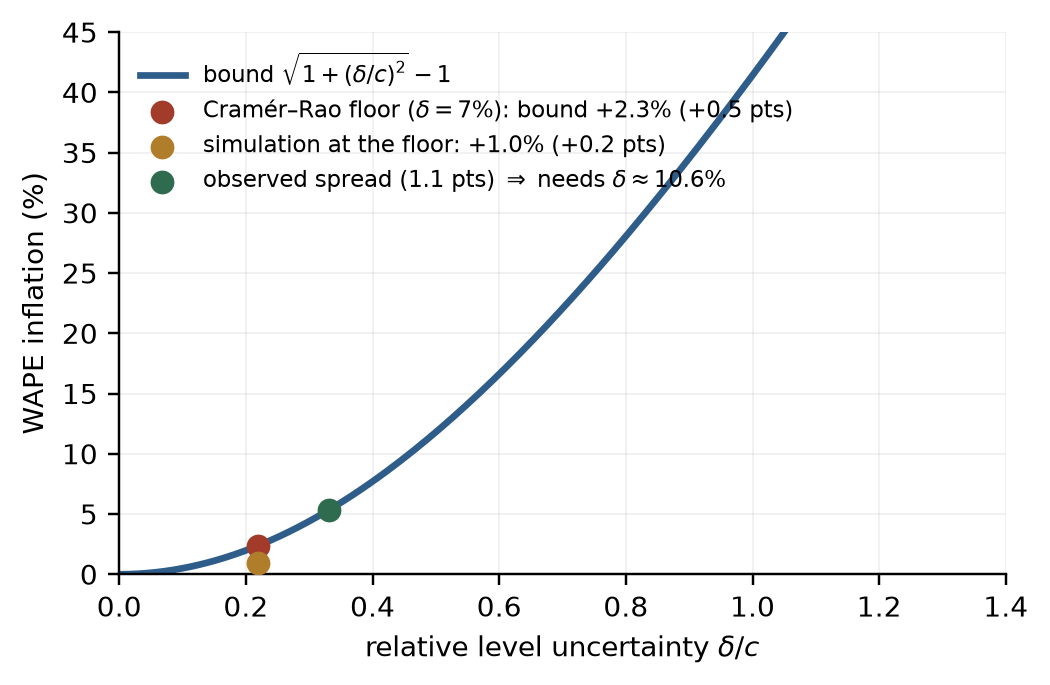
\includegraphics[width=.8\linewidth]{p3_wape_budget.png}
\caption{What a level error costs in WAPE. The bound is a curve; the three
quantities the paper compares are points on it. The Cram\'er--Rao floor permits
$+2.3\%$ inflation, the matched simulation measures $+1.0\%$, and the observed
spread between the honest methods ($5.4\%$) would require a level error of about
$10.6\%$---one and a half times the floor.}
\label{fig:budget}
\end{figure}

Fig.~\ref{fig:budget} reads those numbers against each other. At the floor the
permitted inflation is 2.3\%; the matched simulation measures 1.0\%; and the
\emph{observed} spread between the honest methods is 5.4\%, which the curve says
would require a level error of about 10.6\%---1.5$\times$ the floor. Level
uncertainty could explain the whole spread only if the effective level error were
half again the largest any unbiased estimator can be forced into; at the floor it
explains under half of the spread, and the simulation says a fifth.

The correlation of $0.94$ between $|\text{bias}|$ and WAPE is real
but confounded: rescaling the naive pipeline's forecasts by 1.076 removes its
entire $-7.5\%$ bias and recovers 0.3 of a 2.1-point gap, because the remaining
error comes from a corrupted \emph{history}, not a corrupted level.

\textbf{The asymmetry is what should worry an operator.} A $-7\%$ level error
costs nothing in L1 ($-0.13$ points: it moves predictions toward the median,
where L1 is minimised), while a $+10\%$ error costs 1.6. Biased low is free for
accuracy and expensive for shelves. A pipeline that reports WAPE is structurally
inclined to under-forecast, which is the direction that empties shelves.

The claim makes two falsifiable predictions. (i) No honest method should reach
about 17 WAPE on this protocol: the level carries at most a couple of points, and
it is already corrected. (ii) A method that beats the floor by a wide margin is
more likely leaking the holdout than exploiting information that the Fisher
bound says is not in the data.

The run-to-run noise is the same size as the effect: SAITS scored 20.70, 21.46,
21.64 and 21.70 over four seeds, so the between-method spread (1.1) is comparable
to the within-model spread (1.0). Ranking methods on one run of this benchmark is
not informative at the resolution the literature reports.

A foundation model lands on the same floor. Zero-shot Chronos-Bolt
\citep{ansari2024} on raw sales scores 23.4 WAPE with a $-9.8\%$ bias---worse than
a plain gradient-boosted model, because it consumes the capped series and has no
channel for the stock-out flag. Fed a de-censored history it scores 20.6 with
$-4.2\%$. The model changed the level it was shown, and the level is the only
thing that moved: 23.4 to 20.6 is the bias, not a modelling gain.

\section{What is not bounded}

Under a 50:1 shortage-to-holding ratio, ordering at the newsvendor quantile
$q^{*}\approx0.98$ instead of at the mean moves lost units from 6139 to 365
($16.8\times$) for the naive pipeline, and from 5507 to 329 ($16.7\times$) once
the history is de-censored; at a \emph{fixed} quantile the choice of
reconstruction moves them by 10--21\%. The corner-to-corner number,
$18.7\times$, combines the two moves, and the decomposition is worth keeping
straight: the decision is worth an order of magnitude, the estimation inside it a
tenth of that.

\begin{table}[h]
\centering\small
\caption{Lost units against the ordering quantile. The policy and the 50:1 cost
ratio are identical in every cell; reading down a column is the decision, reading
across a row is the reconstruction.}
\label{tab:quantile}
\begin{tabular}{lrrr}
\toprule
ordering quantile & sales as demand & Tobit (severity) & NB (severity) \\
\midrule
0.50 (the mean) & 6139 & 5507 & 4864 \\
0.90 & 1186 & 1025 & 848 \\
0.95 & 669 & 608 & 533 \\
0.98 (newsvendor) & 365 & \textbf{329} & 342 \\
\bottomrule
\end{tabular}
\end{table}

\begin{figure}[t]
\centering
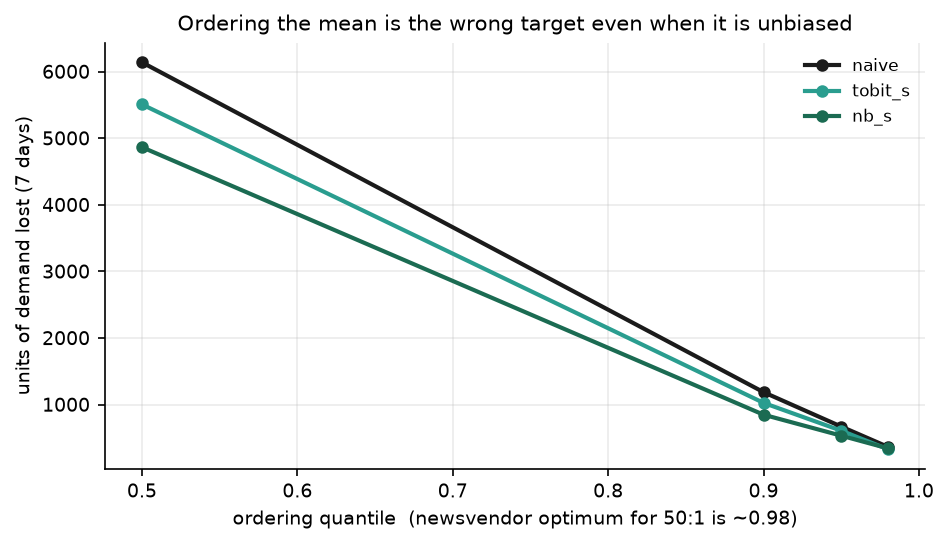
\includegraphics[width=.75\linewidth]{r4_quantile.png}
\caption{Lost units against the ordering quantile. The curves are roughly
parallel: the quantile sets the level, the reconstruction shifts it by a constant
fraction.}
\label{fig:quantile}
\end{figure}

Two readings of the grid matter. \emph{Down a column}, the quantile is worth
14.2$\times$ to 16.8$\times$ in lost units. \emph{Across a row}, at a fixed
quantile, the entire reconstruction question is worth 10--21\%, and at the
newsvendor quantile 10\%. The decision dominates the estimation by an order of
magnitude and---unlike the estimation---is not bounded by the information the
censoring destroyed. That the point forecast is the wrong target under asymmetric
cost is textbook \citep{gneiting2014,petropoulos2022,talluri2004}; what the
information bound adds is the ratio between the two layers.

\section{Can the mask be optimised instead?}

If censoring destroys information, the obvious response is to stock more and
observe more. We test it in a Bayesian simulation: 300 SKUs, 30 weeks, NB2 demand
with an unknown level, three policies---greedy (newsvendor quantile), dither
(same mean inventory, $\pm40\%$ randomisation) and explore ($+1$ posterior
sd)---against an inventory-matched greedy control.

\begin{table}[h]
\centering
\small
\caption{Posterior error after 30 weeks, fill rate and mean inventory.}
\label{tab:dc}
\begin{tabular}{lrrr}
\toprule
policy & posterior error & fill & mean inventory \\
\midrule
greedy $q=0.91$ & 21.1\% & 0.783 & 3.06 \\
dither & 21.5\% & 0.731 & 3.00 \\
explore & 16.3\% & 0.837 & 3.37 \\
greedy $q=0.995$ (matched) & 17.1\% & 0.830 & 3.31 \\
\bottomrule
\end{tabular}
\end{table}

Randomisation at fixed inventory buys nothing, and once inventory is matched,
exploration buys 0.8 pp. At scalar uncertainty, information gathering has no
separate value: the lever \emph{is} the inventory level. The information cannot
be cheaply bought back, which is why the bound in \S2 is a constraint rather than
a modelling inconvenience.

\section{What this changes}

\textbf{Measure aggregate bias first.} It is the whole of the WAPE difference and
it is cheap to compute from a clean holdout week. A pipeline that reports WAPE
but not bias reports the bounded part and omits the unbounded one.

\textbf{Correct it with the cheapest correct estimator.} The severity-weighted
likelihood needs the stock-status log and fifteen seconds of CPU; it takes a
$-7.1\%$ bias to $-0.3\%$. Deep imputation reaches $+2.1\%$ at three orders of
magnitude more compute, with run-to-run variance larger than the remaining gap.

\begin{figure}[t]
\centering
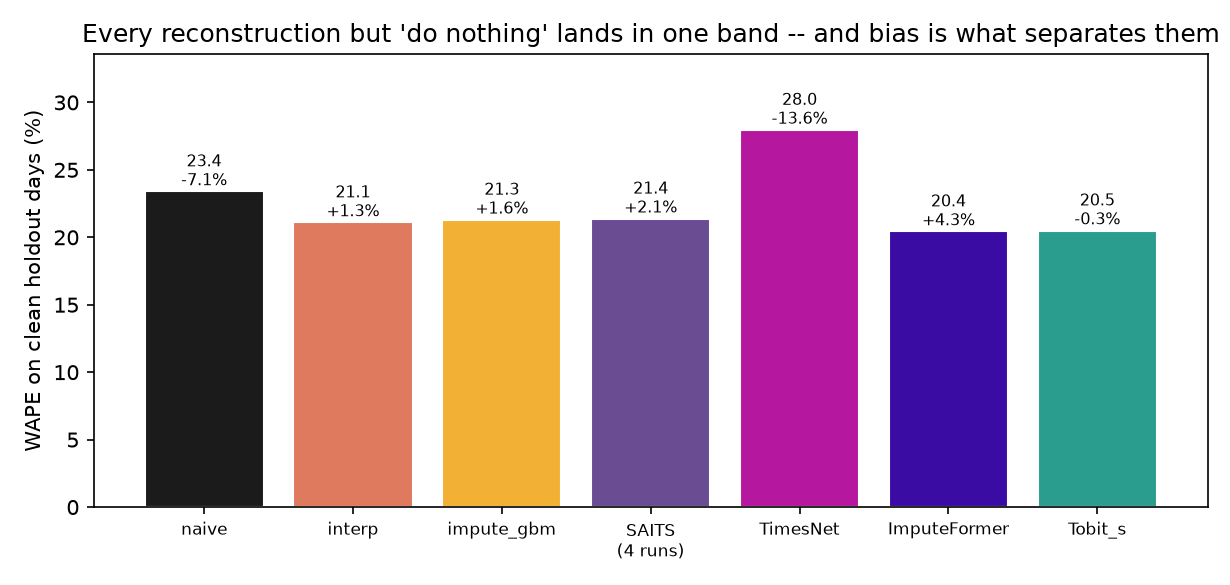
\includegraphics[width=.8\linewidth]{r6_deep_imputer.png}
\caption{The arithmetic of the previous paragraph as a picture: the deep imputers
cost 325--900\,s of CPU and land within 1.1 WAPE of a likelihood that costs
15\,s, with a larger bias in every case (SAITS $+2.1\%$, ImputeFormer $+4.3\%$,
a normalised TimesNet $-13.6\%$, against $-0.3\%$ for the severity-weighted
Tobit). The vertical distance to the floor is noise; the horizontal distance is
three orders of magnitude.}
\label{fig:deep}
\end{figure}

Fig.~\ref{fig:deep} prices that trade. A team is entitled to spend three orders of
magnitude of compute on two tenths of a WAPE point, but it should do so knowing
that the reconstruction was never the expensive part of the problem, and that the
bias it buys is larger in every deep case than the fifteen-second estimator's.

\textbf{Spend the next dollar on the quantile.} No information bound applies to
the ordering rule; it is worth 14.2--16.8$\times$ in lost units for a fixed
estimator (16.8--18.7$\times$ if the history is de-censored too), against
10--21\% for the entire reconstruction question.

\textbf{Carry the 7\%.} The floor is a property of the data and is not removable,
but it is small next to the 25\% daily variability that already drives safety
stock. Per-SKU level uncertainty is a second-order term in inventory sizing, and
should be acknowledged rather than modelled.

\subsection{The ladder: censoring is a procurement decision}

The bound is a property of the data rather than of the model, which turns
de-censoring from a modelling question into a procurement one. What can be
recovered is fixed by what is logged:

\begin{table}[h]
\centering\small
\caption{What each rung of the logging ladder buys. Bias measured on the
official holdout, scored on fully-stocked days.}
\label{tab:ladder}
\begin{tabular}{lll r}
\toprule
rung & you log & the correction you can justify & bias \\
\midrule
R0 & sales & nothing: the censoring is unidentifiable & unknown \\
R1 & + a stock-out flag & the textbook censored likelihood & $+9.4$ to $+28.0\%$ \\
R2 & + stock-out hours & severity-weighted likelihood & $-0.3\%$ \\
R3 & + hourly sales & same, self-calibrated profile & $-0.3\%$ \\
\bottomrule
\end{tabular}
\end{table}

R1 to R2 is one column in the warehouse system, and it is worth 10--28 points of
bias---more than every modelling advance reported on this benchmark combined,
this paper's included.

\subsection{What the audit reports}

The accompanying tool answers the three questions in the order they are asked:
how censored is this table (rate, severity, effective days, the 7\% floor); what
was demand (severity-weighted reconstruction, damped for the R1 case because a
full correction over-shoots); and how much to order (the newsvendor quantile of
the predictive distribution). It repairs the predictable failures of real
exports---GBK encodings, renamed columns, duplicate rows, returns arriving as
negative units---and distinguishes a day with no sale from a day with no record,
which the usual pipeline silently conflates by writing a zero.

\paragraph{Code and data.} The dataset is public (CC-BY-4.0). The audit tool,
the estimators, the experiment scripts and every figure here reproduce from one
command on a laptop CPU---no GPU, no training, twelve tests covering both the
estimators and the data-repair layer.

\section{Limitations}

\begin{enumerate}\itemsep2pt
\item $\rho$ assumes a negative-binomial family. Dispersion barely matters, so
the bound is robust to a mis-specified tail, but a zero-inflated process would
change the curve.
\item The bound is for per-SKU estimation from that SKU's own history. A pooled
model borrows strength across series and is not bounded by it; every published
de-censoring method reconstructs series independently, so the bound does apply to
the paradigm compared.
\item The bridge from the bound to the WAPE floor has an analytic form (\S4) and
two simulations behind it; what remains borrowed rather than proved is the
constant at the benchmark's base WAPE, and the $0.94$ correlation is confounded
and is reported as such.
\item Seven holdout days, one split, 90-day window, one country and category.
\item Lead time 3 days, cost ratio 50:1, no shelf life.
\item The dual-control test is a simulation, not a field experiment.
\end{enumerate}

\appendix
\section{The controlled simulator}
\label{app:sim}

Forty SKUs over 420 days are drawn from a negative-binomial level process with a
lognormal scale, a linear trend, weekly and annual sinusoids and 2\% promotion
spikes. Censoring is generated by a daily-review $(s,S)$ policy with a 3-day lead
time, sized on true demand so availability is independent of any forecaster under
test. E1 sweeps the cover; E2 resizes the policy each week from the method's own
forecast; E3 injects a $+35\%$ level shift at day 380 and freezes the forecaster
at day 300.

\section{Run-to-run variance of the deep imputer}
\label{app:variance}

The four SAITS runs quoted in Table~\ref{tab:methods} use one configuration and
four seeds:

\begin{table}[h]
\centering\small
\caption{One SAITS configuration, four seeds.}
\label{tab:seeds}
\begin{tabular}{lrr}
\toprule
run & WAPE & bias \\
\midrule
seed 0 & 20.70 & $+0.0\%$ \\
seed 1 & 21.46 & $+1.7\%$ \\
seed 2 & 21.64 & $+2.7\%$ \\
seed 3 & 21.70 & $+4.1\%$ \\
\bottomrule
\end{tabular}
\end{table}

The within-model range (1.0 WAPE) is the same size as the between-method spread of
the honest methods (1.1). This is why Table~\ref{tab:methods} carries the
inventory columns and bias instead of a leaderboard rank: at one run, at this
resolution, the ranking is not stable, and a paper that reports only the rank is
reporting noise.

A second reproducibility note: the full pipeline (Table~\ref{tab:methods}, the
quantile grid of \S5 and every figure) runs in 300\,s on a laptop CPU with no GPU
and no training, and twelve tests cover the estimators and the data-repair layer.
In a shell that forbids named pipes---some sandboxes do---the run needs
\texttt{JOBLIB\_MULTIPROCESSING=0} and fits serially at about twice the
wall-clock time.

\bibliographystyle{plainnat}
\bibliography{refs}

\end{document}
